\documentclass[conference]{IEEEtran}
\usepackage[utf8]{inputenc}
\usepackage[spanish]{babel}
\usepackage{graphicx}
\usepackage{amsmath, amssymb}
\usepackage{hyperref}
\usepackage{cite}
\usepackage{booktabs}
\usepackage{array}
\usepackage{multirow}
\usepackage{fancyhdr}
\usepackage{lastpage}
\usepackage{longtable}
\usepackage{enumitem}
\usepackage{longtable}
\usepackage{array}
\usepackage{booktabs}

\title{Predicción de Potencia Eólica mediante Ensembles de Machine Learning: Un Enfoque Comparativo}

\author{
	\IEEEauthorblockN{Luis Koc}
	\IEEEauthorblockA{luis.koc@gmail.com}
	\and
	\IEEEauthorblockN{Alex Mancilla}
	\IEEEauthorblockA{afmancilla@gmail.com}
	\and
	\IEEEauthorblockN{Herbert García}
	\IEEEauthorblockA{hamg.94@gmail.com}
	\and
	\IEEEauthorblockN{Denis Paitán}
	\IEEEauthorblockA{denniskano@gmail.com}
}

% Afiliación común centrada a lo ancho
\IEEEoverridecommandlockouts
\IEEEaftertitletext{%
\begin{center}
\vspace{-1.5em}
	\begin{minipage}{\textwidth}
	\centering
	\textit{Facultad de Ingeniería Industrial y de Sistemas\\
	Universidad Nacional de Ingeniería\\
	Lima, Perú}
		\end{minipage}
\vspace{0.5em}
	\end{center}
}

\begin{document}
	
% Configuración de paginación
\pagestyle{fancy}
\fancyhf{}
\fancyhead[L]{\small Predicción de Potencia Eólica mediante Ensembles de ML}
\fancyhead[R]{\small Página \thepage\ de \pageref{LastPage}}
\renewcommand{\headrulewidth}{0.4pt}
\fancyfoot[C]{\thepage}
\renewcommand{\thesubsection}{\Alph{subsection}}

\maketitle

\begin{abstract}
La predicción de la producción horaria en parques eólicos es esencial para garantizar la estabilidad del sistema eléctrico, reducir penalizaciones por desvío y facilitar la integración de energías renovables en el mercado diario. Este estudio desarrolla un modelo de aprendizaje automático con horizonte de 24 horas, basado en un enfoque integral que incluye limpieza avanzada de datos, ingeniería y selección automatizada de características, y ensamblaje de modelos. Se analizaron múltiples algoritmos supervisados —entre ellos \textit{Random Forest}, \textit{Gradient Boosting}, \textit{XGBoost}, \textit{LightGBM}, \textit{CatBoost} y redes neuronales MLP—, integrados mediante técnicas de ensamblado (\textit{stacking} y combinación ponderada). Adicionalmente, se incorporó un sistema de detección no supervisada de anomalías basado en DBSCAN aplicado sobre los residuos del modelo.
		
El mejor desempeño se obtuvo con un \textit{ensemble} ponderado (90\,\% MLP y 10\,\% regresión lineal), que alcanzó un coeficiente de determinación \( R^2 = 0.8234 \) y un error absoluto medio (MAE) de 0.4287. Estos resultados superan a los modelos individuales, validando la eficacia de los métodos \textit{ensemble} para la predicción operativa de potencia eólica. La metodología propuesta es consistente con las mejores prácticas encontradas en la literatura, como el uso de modelos híbridos dinámicos, optimización de pesos mediante algoritmos de enjambre, y reducción de errores mediante clasificación previa de los datos o corrección de predicciones meteorológicas. Se recomienda su implementación práctica y actualización diaria para mejorar la precisión y robustez en escenarios reales de operación.\\
\end{abstract}

\begin{IEEEkeywords}
component, formatting, style, styling, insert
\end{IEEEkeywords}

	
\section{Introducción}
	
La integración de fuentes renovables en la matriz energética contemporánea conlleva desafíos significativos, especialmente debido a la variabilidad inherente de recursos como la energía eólica. La capacidad de anticipar con precisión la generación eléctrica en parques eólicos es crucial para una planificación operativa eficiente, el diseño de estrategias de mantenimiento predictivo y una participación efectiva en mercados eléctricos competitivos. Este trabajo aborda el problema de predicción de potencia eólica mediante un enfoque metodológico integral que combina técnicas avanzadas de aprendizaje automático con análisis exploratorio y procesamiento riguroso de datos.
	
La metodología propuesta contempla un pipeline completo de preprocesamiento que gestiona datos faltantes, detecta y filtra valores atípicos, y aplica escalamiento estandarizado. Asimismo, se implementa un sistema de selección automática de características que combina análisis de correlación, importancia de atributos mediante \textit{Random Forest} y técnicas de \textit{permutation importance}, con el objetivo de identificar las variables más influyentes para el modelo de predicción.
	
\subsection{Contexto y Motivación}
	
La transición hacia un modelo energético bajo en carbono ha posicionado a la energía eólica como una de las tecnologías clave para la descarbonización del sector eléctrico. No obstante, la naturaleza intermitente del recurso eólico introduce incertidumbre y complejidad en la gestión de la red, requiriendo sistemas de pronóstico altamente precisos para reducir costos de operación, evitar penalizaciones por desvío y mejorar la integración con otras fuentes.
	
Los parques eólicos modernos generan grandes volúmenes de datos meteorológicos y operativos que, debidamente procesados, permiten construir modelos predictivos más robustos. La fusión de múltiples fuentes, como datos satelitales (NASA POWER) y mediciones en sitio, posibilita una representación más precisa del entorno operativo, elevando el potencial predictivo de los modelos de aprendizaje automático.
	
\subsection{Objetivos del Trabajo}
	
Los principales objetivos de esta investigación son:
	
\begin{enumerate}
\item Desarrollar un pipeline de preprocesamiento que integre múltiples fuentes de datos meteorológicos y operativos.

\item Aplicar técnicas avanzadas de selección de variables para identificar los atributos más relevantes en la predicción de potencia.

\item Evaluar el desempeño de diversos algoritmos de \textit{machine learning}, incluyendo modelos de ensamblado y redes neuronales profundas.

\item Implementar un sistema de detección de anomalías que identifique condiciones operativas atípicas.

\item Validar la capacidad predictiva del modelo para un horizonte de 24 horas.
\end{enumerate}
	
\subsection{Contribuciones Principales}
	
Las contribuciones de este trabajo al estado del arte en predicción de potencia eólica incluyen:
	
\begin{itemize}
\item Un pipeline robusto de preprocesamiento que gestiona eficazmente valores ausentes y atípicos.

\item Un sistema combinado de selección automática de características que optimiza la dimensionalidad del conjunto de datos.

\item Una evaluación comparativa de modelos clásicos y avanzados de \textit{machine learning}, incluyendo técnicas de ensamblado.

\item Un enfoque de \textit{ensemble} ponderado que mejora el desempeño respecto a modelos individuales.

\item Un sistema de detección de anomalías basado en DBSCAN, útil para diagnosticar errores operativos o condiciones meteorológicas excepcionales.

\end{itemize}

\section{Estado del Arte}

Este estudio se basa en una revisión exhaustiva de 18 artículos recientes sobre predicción de potencia eólica, los cuales exploran diferentes enfoques, modelos y atributos relevantes. A continuación, se resumen las principales tendencias detectadas y aquellas adoptadas en el presente trabajo.

\subsection{Atributos Recurrentes}

\begin{itemize}
	\item \textbf{Velocidad del viento:} Es el predictor más común y crítico. Se mide a distintas alturas (10m, 90m, 100m) y a menudo se utiliza su cuadrado o cubo para capturar relaciones no lineales conforme a la ley de Betz.
	
	\item \textbf{Temperatura del aire:} Considerada para ajustar efectos atmosféricos. En este estudio, la temperatura a 2 metros (NASA) resultó ser la variable más influyente.
	
	\item \textbf{Presión atmosférica y humedad relativa:} Frecuentemente usadas para enriquecer el contexto meteorológico. Aplicadas en estudios como Liu et al. (2023), Rathnayake et al. (2025) y Jonkers et al. (2024).
	
	\item \textbf{Lags temporales:} Variables como \textit{Lag-1} y \textit{Lag-24} de velocidad del viento capturan la dinámica y la inercia del sistema. Se incorporan en este estudio como atributos derivados.
	
	\item \textbf{Estadísticas móviles:} Promedios y desviaciones estándar móviles ayudan a suavizar el ruido y detectar tendencias. Inspirado en trabajos como Cococcioni et al. (2012) y Huang et al. (2023).
\end{itemize}

\subsection{Modelos de Predicción Utilizados}

\begin{itemize}
	\item \textbf{Modelos Lineales:} La regresión lineal es ampliamente empleada como referencia base en múltiples investigaciones.
	
	\item \textbf{Ensemble de Árboles:} Random Forest, Extra Trees y Gradient Boosting aparecen como alternativas robustas y de bajo sobreajuste.
	
	\item \textbf{Boosting Avanzado:} Algoritmos como XGBoost, LightGBM y CatBoost presentan altos niveles de precisión. Adoptados especialmente en estudios como Tsai et al. (2023), Bouabdallaoui et al. (2023) y Tuncar et al. (2024).
	
	\item \textbf{Redes Neuronales:} Modelos MLP, LSTM y CNN se consolidan en estudios recientes por su capacidad para capturar relaciones no lineales y temporales complejas. En este trabajo se integró un MLP como componente principal del ensemble.
	
	\item \textbf{Modelos Combinados:} Técnicas de combinación como \textit{stacking}, \textit{bagging} o \textit{weighted ensembles} permiten aprovechar múltiples paradigmas. En este estudio, el mejor modelo fue un ensemble ponderado MLP (90\%) + regresión lineal (10\%).
\end{itemize}

\subsection{Contribuciones Adoptadas}

\begin{itemize}
	\item Selección de atributos derivados de estudios previos, incluyendo transformaciones polinómicas y características temporales.
	
	\item Limpieza exhaustiva de datos utilizando IQR, z-score y reglas físicas del dominio, tal como se sugiere en trabajos como Kolev y Sulakov (2019) y Jonkers et al. (2024).
	
	\item Integración de múltiples fuentes meteorológicas (NASA POWER y OpenMeteo), siguiendo buenas prácticas observadas en Liu et al. (2023).
	
	\item Implementación de un pipeline completo con imputación iterativa basada en Random Forest, selección automática de características, y evaluación de múltiples algoritmos.
	
	\item Aplicación de PCA y DBSCAN para detección de anomalías, identificando registros con errores de predicción extremos, técnica inspirada en Huang et al. (2023).
	
	\item Validación sobre datos del día siguiente, evaluando la capacidad de generalización del modelo, en línea con el enfoque de Jonkers et al. (2024).
\end{itemize}


\begin{table}[htbp]
	\caption{Comparación de Resultados entre Estudios Relevantes}
	\centering
	\begin{tabular}{@{}lccc@{}}
		\toprule
		\textbf{Estudio} & \textbf{Modelo} & \textbf{MAE} & \textbf{R\textsuperscript{2}} \\ \midrule
		Huang et al. (2023)     & RF+GB+SVM+KNN   & 5.15       & 0.93 \\
		Bouabdallaoui et al. (2023) & MLP                  & 5.3        & 0.92 \\
		Kolev y Sulakov (2019)  & Gradient Boosting     & 6.02 MW    & 0.77 \\
		\textbf{Este trabajo}   & \textbf{MLP + LR (90/10)} & \textbf{0.43} & \textbf{0.82} \\
		\bottomrule
	\end{tabular}
	\label{tab:comparacion-resultados}
\end{table}


	
\subsection{Importancia y motivación}
	
Liu et al.~\cite{liu2023day} destacan la importancia crítica de contar con modelos de predicción robustos y precisos en contextos de mercados eléctricos regulados, donde los errores de pronóstico pueden generar penalizaciones económicas significativas. Esta motivación es consistente con nuestro trabajo, que busca anticipar la potencia horaria con 24 horas de antelación para optimizar la operación del parque y evitar desvíos en la oferta energética.
	
Chen y Folly~\cite{chen2018wind} presentan una taxonomía completa de métodos de predicción eólica, clasificándolos por horizonte temporal (corto, medio y largo plazo) y por tipo de metodología (estadística, física, híbrida y basada en inteligencia artificial). Su marco conceptual guía la organización de esta sección y justifica la elección de enfoques híbridos y de ML en nuestro proyecto.
	
\subsection{Modelos físicos y numéricos}
	
Los modelos físicos como CFD o mesoescala (WRF) son útiles para representar fenómenos atmosféricos, aunque suelen ser costosos computacionalmente. Jacondino et al.~\cite{jacondino2021hourly} demostraron que el esquema de parametrización de la capa límite (BouLac) en WRF influye significativamente en la precisión del pronóstico horario (MAE ~12.6\%). En nuestro caso, los datos meteorológicos de Open-Meteo y NASA POWER actúan como entradas de alta resolución que cumplen una función análoga, pero integrados a modelos de ML más ligeros y prácticos para operación diaria.
	
\subsection{Modelos estadísticos}
	
Qureshi et al.~\cite{qureshi2023shortterm} compararon ARIMA y GRU en un parque eólico de Pakistán, reportando un RMSE de 0.047 y \(R^2 = 0.89\) a favor del modelo GRU. Esto evidencia la limitación de los modelos lineales para capturar la no linealidad del recurso eólico. Este hallazgo motivó la inclusión de modelos no lineales en nuestra comparación, como redes MLP y modelos ensemble.
	
\subsection{Aprendizaje automático y redes profundas}
	
El uso de algoritmos como Random Forest y Gradient Boosting se ha consolidado como estándar en predicción eólica. Kolev y Sulakov~\cite{kolev2019forecasting} muestran que MLP, RBF y FNN superan consistentemente a modelos físicos para predicción day-ahead, validando la efectividad de técnicas basadas en datos.
	
Ayene y Yibre~\cite{ayene2024wind} implementaron LSTM, Bi-LSTM y GRU con datos de 5 minutos, logrando \(R^2 > 0.97\), evidenciando la capacidad de las redes recurrentes para capturar patrones temporales. Aunque nuestro trabajo opera a una resolución horaria, estos resultados respaldan la selección de arquitecturas neuronales para tareas temporales.
	
\subsection{Ensembles y optimización}
	
Huang et al.~\cite{huang2023ensemble} presentan un enfoque de ensemble optimizado mediante algoritmos de enjambre (PSO, SSA, WOA), logrando mejoras de hasta 31\% frente a modelos individuales. Además, emplean Random Forest para corregir errores en las predicciones de velocidad del viento, estrategia análoga a nuestro uso de variables derivadas y ensamblados ponderados.
	
Rathnayake et al.~\cite{rathnayake2025predicting} validaron 24 algoritmos en el parque Musalpetti (Sri Lanka), encontrando que los modelos bagging y stacking alcanzan mayor estabilidad y precisión. Este estudio refuerza nuestra decisión de combinar MLP y regresión lineal en un ensemble ponderado que logró \(R^2 = 0.823\), superando a todos los modelos individuales.
	
\subsection{Selección de características y preprocesamiento}
	
La correcta selección de variables es clave para evitar sobreajuste y mejorar la interpretabilidad. AlShafeey y Csaki~\cite{alshafeey2024adaptive} proponen un sistema adaptativo que elige dinámicamente el mejor modelo y conjunto de variables según la ventana temporal. Este enfoque motivó nuestro uso combinado de análisis de correlación, importancia de características vía Random Forest y \textit{permutation importance}, seleccionando 9 variables relevantes.
	
Cococcioni et al.~\cite{cococcioni2012oneday} aplican SVM y MLP para predicción día-ahead en plantas solares, resaltando la necesidad de un preprocesamiento riguroso. En línea con ello, nuestro pipeline incluye detección de outliers (z-score e IQR), filtrado físico velocidad-potencia, y escalamiento estandarizado.
	
\subsection{Detección de anomalías}
	
La identificación de valores atípicos es clave para evitar la degradación del modelo. DBSCAN, Isolation Forest y One-Class SVM son técnicas comunes. Nuestro uso de DBSCAN sobre residuos de predicción sigue el enfoque de Huang et al.~\cite{huang2023ensemble} y nos permitió aislar un 5.9\% de puntos anómalos que correspondían a errores de lectura o condiciones excepcionales, mejorando así la estabilidad del modelo.
	
\subsection{Tendencias actuales}
	
Las líneas de investigación más relevantes en predicción eólica incluyen:
	
\begin{itemize}

\item Fusión de múltiples fuentes de datos (satélite, estaciones, reanálisis).

\item Uso de \textit{transfer learning} para generalizar modelos a nuevos parques.

\item Modelos probabilísticos que predicen intervalos, no solo valores puntuales.

\item Incorporación de técnicas interpretables como SHAP para explicar predicciones.

\item Automatización de pipelines con actualización diaria y autoentrenamiento.
\end{itemize}
	
Estas tendencias están alineadas con nuestro trabajo, que propone un enfoque modular, explicable (mediante importancia de variables) y operativo, capaz de integrarse en un flujo de producción energética diaria.
	
\subsection{Otros Estudios Relevantes}
	
Además de los trabajos ya discutidos, se revisaron otros 13 estudios significativos que complementan y refuerzan la metodología adoptada en esta investigación. A continuación, se resumen sus principales aportes agrupados por tipo de contribución:
	
\textbf{Modelos comparativos y validaciones extensas}:
\begin{itemize}[leftmargin=*,itemsep=1pt]
\item \textbf{Bouabdallaoui et al. (2023)} comparan cuatro modelos de ML, destacando el rendimiento de RF y ANN en horizontes cortos.

\item \textbf{Qureshi et al. (2023)} muestran que GRU supera a ARIMA significativamente (\(R^2 = 0.89\)), confirmando la efectividad de redes recurrentes.

\item \textbf{Rathnayake et al. (2025)} evalúan 24 algoritmos y resaltan el stacking y bagging como enfoques robustos.
\end{itemize}
	
\textbf{Técnicas avanzadas de ensamblado y optimización}:
\begin{itemize}[leftmargin=*,itemsep=1pt]
\item \textbf{Huang et al. (2023)} implementan ensamblados optimizados por enjambre (PSO, SSA, WOA), mejorando hasta un 31\% sobre modelos base.

\item \textbf{Huang et al. (2023b)} proponen un ensamblado con 25 submodelos y reducción de error de hasta 12–31\%.
\end{itemize}
	
\textbf{Modelos de redes profundas}:
\begin{itemize}[leftmargin=*,itemsep=1pt]

\item \textbf{Ayene y Yibre (2024)} usan LSTM, Bi-LSTM y GRU con datos cada 5 minutos, logrando \(R^2 > 0.97\).

\item \textbf{Jonkers et al. (2024)} desarrollan una CNN profunda para predicción regional y probabilística con gran precisión.

\end{itemize}
	
\textbf{Preprocesamiento y calidad de datos}:
\begin{itemize}[leftmargin=*,itemsep=1pt]

\item \textbf{Cococcioni et al. (2012)} enfatizan el rol del preprocesamiento al predecir en instalaciones solares usando MLP y SVR.

\item \textbf{Kirk-Davidoff (2012)} refuerza la comprensión física del viento, útil para filtrar valores atípicos y anomalías.

\end{itemize}
	
\textbf{Revisiones y tendencias metodológicas}:
\begin{itemize}[leftmargin=*,itemsep=1pt]

\item \textbf{Chen y Folly (2018)}, \textbf{Tsai et al. (2023)} y \textbf{Tuncar et al. (2024)} presentan revisiones de técnicas de predicción, clasificando por horizonte, modelo y aplicación.

\item \textbf{AlShafeey y Csaki (2024)} introducen un modelo adaptativo que selecciona dinámicamente el mejor algoritmo, enfoque inspirador para diseños futuros.

\end{itemize}
	
\subsection{Otros Estudios Relevantes}
	
Además de los estudios centrales discutidos previamente, se analizaron otros trabajos recientes que aportan elementos clave para la construcción metodológica de esta investigación. A continuación, se presentan sus principales contribuciones, organizadas por temática y con énfasis en cómo fortalecen las decisiones adoptadas en este estudio.
	

\textbf{Modelos comparativos y validaciones extensas}:
\begin{itemize}[leftmargin=*,itemsep=1pt]

\item \textbf{Bouabdallaoui et al. (2023) \cite{bouabdallaoui2023application}} comparan cuatro algoritmos (MLP, RF, SVR, RBF) para predicción de corto plazo, concluyendo que RF y MLP son los más robustos ante datos meteorológicos volátiles, lo cual valida la inclusión de estos modelos en nuestro conjunto evaluado y su uso en ensembles.

\item \textbf{Qureshi et al. (2023) \cite{qureshi2023shortterm}} destacan la superioridad de GRU sobre ARIMA en predicciones de viento, con \(R^2 = 0.89\), evidenciando la ventaja de modelos no lineales secuenciales. Esto respalda la exploración futura de arquitecturas tipo GRU o LSTM en nuestros pipelines.

\item \textbf{Rathnayake et al. (2025) \cite{rathnayake2025predicting}} realizan una comparación masiva de 24 algoritmos ML sobre datos reales del parque Musalpetti, demostrando que los enfoques basados en \textit{stacking} y \textit{bagging} ofrecen mejor estabilidad, lo cual refuerza nuestra elección de ensembles ponderados como solución final.

\end{itemize}
	
\textbf{Técnicas avanzadas de ensamblado y optimización}:
\begin{itemize}[leftmargin=*,itemsep=1pt]

\item \textbf{Huang et al. (2023) \cite{huang2023ensemble}} implementan un método de ensamblado ponderado optimizado con algoritmos de enjambre (PSO, SSA, WOA), logrando una mejora de hasta 31\% sobre modelos individuales. Su enfoque inspiró nuestra estrategia de combinación de MLP con regresión lineal como ensemble final.

\item \textbf{Huang et al. (2023b) \cite{huang2023multiobjective}} amplían esta estrategia tilizando 25 submodelos en un ensamblado jerárquico, logrando reducir el error en un rango de 12–31\%. Su aproximación reafirma el potencial de ensamblados multi-nivel, que podría implementarse en investigaciones futuras.

\end{itemize}


\textbf{Modelos de redes profundas}:
\begin{itemize}[leftmargin=*,itemsep=1pt]

\item \textbf{Ayene y Yibre (2024) \cite{ayene2024wind}} implementan LSTM, Bi-LSTM y GRU para predicción de 5 minutos en un parque eólico, alcanzando \(R^2 > 0.97\). Sus resultados sugieren que la inclusión de memoria de largo plazo en redes neuronales es crucial en series temporales densas, lo que abre posibilidades para modelos más sofisticados en trabajos futuros.

\item \textbf{Jonkers et al. (2024) \cite{jonkers2024probabilistic}} desarrollan una arquitectura CNN profunda combinada con codificadores espaciales y técnicas probabilísticas, logrando predicción regional de alta precisión. Su enfoque valida el uso de datos multiespacio-temporales y modelado probabilístico como extensiones viables a nuestro enfoque determinista.

\end{itemize}


\textbf{Preprocesamiento y calidad de datos}:
\begin{itemize}[leftmargin=*,itemsep=1pt]

\item \textbf{Cococcioni et al. (2012) \cite{cococcioni2012oneday}} demuestran que el preprocesamiento cuidadoso (incluyendo normalización, selección de variables y filtrado físico) mejora notablemente la precisión de MLP y SVR en instalaciones fotovoltaicas. Esto refuerza la importancia de nuestro pipeline de limpieza y selección.

\item \textbf{Kirk-Davidoff (2012) \cite{kirk2012forecasting}} analiza la física del recurso eólico, subrayando cómo errores en mediciones o turbulencias afectan los modelos. Su marco físico respaldó nuestras reglas de filtrado físico de datos en la curva de potencia.

\end{itemize}
	
\textbf{Revisiones y tendencias metodológicas}:

\begin{itemize}[leftmargin=*,itemsep=1pt]

\item \textbf{Chen y Folly (2018) \cite{chen2018wind}}, \textbf{Tsai et al. (2023) \cite{tsai2023review}} y \textbf{Tuncar et al. (2024) \cite{tuncar2024review}} proporcionan revisiones exhaustivas que organizan los enfoques en función del horizonte temporal, complejidad y tipo de datos. Sus clasificaciones sirvieron como base para estructurar nuestro marco comparativo y decidir sobre el uso de ML frente a enfoques físicos.

\item \textbf{AlShafeey y Csaki (2024) \cite{alshafeey2024adaptive}} proponen un sistema adaptativo que selecciona automáticamente el mejor algoritmo y conjunto de variables según la ventana temporal. Este enfoque fue una fuente de inspiración directa para nuestro proceso de selección de características y ponderación de modelos.

\end{itemize}
	
	
\textbf{Complementos específicos y alineamientos con este trabajo}:
\begin{itemize}[leftmargin=*,itemsep=1pt]

\item El modelo híbrido CNN-BiLSTM con autoregresión propuesto en 2024 \cite{zhang2024cnnbilstm} muestra cómo integrar arquitecturas secuenciales con componentes clásicos para robustecer la predicción, estrategia análoga a nuestra combinación MLP + regresión.

\item El enfoque "Adaptive ML" (2024) \cite{alshafeey2024adaptive} propone una lógica de selección dinámica de algoritmos, coherente con nuestro esquema de búsqueda de pesos óptimos en ensembles.

\item Un estudio con WRF en Brasil (2021) \cite{jacondino2021hourly} sustenta el uso de meteorología numérica como fuente externa, lo cual motivó nuestra integración de datos de OpenMeteo y NASA POWER como insumos multifuente.

\item \textbf{Lee et al. (2024) \cite{lee2024vertical}} introducen una técnica novedosa de extracción de características basada en capas verticales del viento, mejorando la representación espacial de datos meteorológicos para predicción day-ahead. Aunque nuestro trabajo no explora directamente perfiles verticales, este enfoque sugiere oportunidades de mejora futura en la integración de datos atmosféricos tridimensionales.
		
\end{itemize}
	
Estos estudios respaldan y enriquecen las decisiones adoptadas en esta investigación, proporcionando validación externa y orientaciones metodológicas para la mejora continua del pipeline de predicción.

	
\section{Metodología}
	
\subsection{Descripción del Conjunto de Datos}

El conjunto de datos utilizado en este trabajo proviene de múltiples fuentes que proporcionan información complementaria sobre las condiciones meteorológicas y operativas del parque eólico. Una descripción detallada de todas las variables se encuentra en el Apéndice A (Tablas \ref{tab:nasa_variables}, \ref{tab:openmeteo_variables}, \ref{tab:operational_variables}, \ref{tab:derived_features}, \ref{tab:selected_features} y \ref{tab:estadisticas_descriptivas}).
	
\subsubsection{Datos Meteorológicos NASA POWER}

La plataforma NASA POWER (Prediction Of Worldwide Energy Resources) proporciona datos meteorológicos de alta resolución temporal y espacial. Los datos incluyen:

\begin{itemize}

\item \textbf{Velocidad del viento}: Medida a diferentes alturas (10m, 90m)

\item \textbf{Temperatura}: Temperatura del aire a 2 metros de altura

\item \textbf{Presión atmosférica}: Presión superficial y a diferentes alturas

\item \textbf{Humedad relativa}: Humedad del aire

\item \textbf{Radiación solar}: Radiación incidente en superficie

\end{itemize}
	
Los datos se descargan con resolución horaria y se procesan para alinear con los timestamps de los datos operativos del parque. Una descripción completa de las variables NASA POWER se presenta en la Tabla \ref{tab:nasa_variables} del Apéndice A.
	
\subsubsection{Datos OpenMeteo}

OpenMeteo proporciona información meteorológica complementaria que incluye:
\begin{itemize}

\item \textbf{Velocidad del viento}: Medida a 10m y 90m de altura

\item \textbf{Temperatura}: Temperatura del aire a 2m

\item \textbf{Presión atmosférica}: Presión superficial

\item \textbf{Humedad relativa}: Humedad del aire

\item \textbf{Precipitación}: Lluvia y nieve

\end{itemize}
	
Esta fuente proporciona datos adicionales que complementan la información de NASA POWER, permitiendo una caracterización más completa de las condiciones meteorológicas. Las variables OpenMeteo se detallan en la Tabla \ref{tab:openmeteo_variables} del Apéndice A.
	
\subsubsection{Datos Operativos del Parque}
Los datos operativos incluyen información en tiempo real sobre el funcionamiento del parque eólico:

\begin{itemize}
\item \textbf{Potencia activa total}: Potencia eléctrica generada por el parque

\item \textbf{Número de aerogeneradores disponibles}: Turbinas en funcionamiento

\item \textbf{Número de aerogeneradores limitados}: Turbinas con restricciones operativas

\item \textbf{Potencia escalada}: Potencia normalizada por número de turbinas disponibles

\end{itemize}
	
Las variables operativas del parque se describen en detalle en la Tabla \ref{tab:operational_variables} del Apéndice A.
	
\subsection{Pipeline de Preprocesamiento}

El preprocesamiento de datos es fundamental para el éxito de los modelos de machine learning. Se implementó un pipeline robusto que incluye las siguientes etapas:
	
\subsubsection{Merge de Fuentes de Datos}

La integración de múltiples fuentes de datos se realiza mediante timestamps, asegurando la sincronización temporal de todas las variables. Se utiliza un merge interno para mantener solo los registros que tienen información completa en todas las fuentes.
	
\subsubsection{Manejo de Valores Faltantes}

Se implementa un sistema de imputación iterativa basado en Random Forest que estima valores faltantes utilizando las relaciones entre variables. Este enfoque es superior a métodos simples como interpolación lineal ya que considera las correlaciones complejas entre variables.
	
\subsubsection{Detección y Eliminación de Outliers}
Se aplican múltiples técnicas para identificar y eliminar valores atípicos:

\begin{enumerate}

\item \textbf{Filtrado por IQR}: Eliminación de valores fuera del rango intercuartílico

\item \textbf{Limpieza por z-score}: Detección de outliers mediante normalización estadística

\item \textbf{Filtros de dominio}: Reglas específicas basadas en conocimiento físico del sistema

\end{enumerate}
	
	Los filtros de dominio incluyen reglas como:
	\begin{itemize}
		\item Eliminar registros donde la potencia es alta pero la velocidad del viento es baja
		\item Eliminar registros donde la velocidad del viento es alta pero la potencia es baja
		\item Eliminar valores negativos de potencia
		\item Eliminar valores de potencia que exceden la capacidad nominal del parque
	\end{itemize}
	
	\subsection{Ingeniería de Características}
	La ingeniería de características es crucial para capturar patrones complejos en los datos. Se generan características adicionales que incluyen:
	
	\subsubsection{Transformaciones Polinómicas}
	Se aplican transformaciones polinómicas a las variables de velocidad del viento para capturar relaciones no lineales:
	\begin{itemize}
		\item \textbf{Cuadráticas}: $v^2$ para capturar efectos cuadráticos
		\item \textbf{Cúbicas}: $v^3$ para capturar efectos cúbicos
	\end{itemize}
	
	Estas transformaciones son especialmente importantes en energía eólica debido a la relación cúbica entre velocidad del viento y potencia (Ley de Betz). Las características derivadas más importantes se presentan en la Tabla \ref{tab:derived_features} del Apéndice A.
	
	\subsubsection{Características Temporales}
	Se incorporan características temporales para capturar dependencias en el tiempo:
	\begin{itemize}
		\item \textbf{Lag-1}: Valor anterior de velocidad del viento
		\item \textbf{Lag-24}: Valor de velocidad del viento de 24 horas antes
	\end{itemize}
	
	Estas características ayudan a capturar patrones diarios y la inercia del sistema.
	
	\subsubsection{Estadísticas Móviles}
	Se calculan estadísticas móviles para suavizar el ruido y capturar tendencias:
	\begin{itemize}
		\item \textbf{Media móvil}: Promedio de los últimos 3 períodos
		\item \textbf{Desviación estándar móvil}: Variabilidad de los últimos 3 períodos
	\end{itemize}
	
	\subsubsection{Características de Interacción}
	Se crean características que combinan información de múltiples fuentes:
	\begin{itemize}
		\item \textbf{Diferencia}: $v_{NASA} - v_{OpenMeteo}$ para capturar discrepancias entre fuentes
		\item \textbf{Producto}: $v_{NASA} \times v_{OpenMeteo}$ para capturar efectos de interacción
	\end{itemize}
	
	\subsubsection{Normalización de Variables}
	Se aplica normalización Min-Max para escalar todas las características al rango [0,1]:
	\begin{equation}
		x_{norm} = \frac{x - x_{min}}{x_{max} - x_{min}}
	\end{equation}
	
	Esta normalización es importante para algoritmos sensibles a la escala como redes neuronales y SVM.
	
	\subsection{Selección Automática de Características}
	La selección de características es fundamental para reducir la dimensionalidad y mejorar la interpretabilidad del modelo. Se implementa un pipeline de tres etapas que combina diferentes técnicas:
	
	\subsubsection{Eliminación por Correlación}
	Se calcula la matriz de correlación de Pearson entre todas las características y se eliminan aquellas con correlación absoluta superior a 0.96. Esto reduce la multicolinealidad y mejora la estabilidad numérica del modelo.
	
	\subsubsection{Selección basada en Importancia}
	Se utiliza SelectFromModel con Random Forest para identificar características con importancia superior a la mediana. Random Forest proporciona una medida robusta de importancia que considera tanto la capacidad predictiva como la estabilidad.
	
	\subsubsection{Permutation Importance}
	Se aplica permutation importance para obtener un ranking final de las características más relevantes. Esta técnica es especialmente útil porque:
	\begin{itemize}
		\item Es independiente del algoritmo de machine learning utilizado
		\item Proporciona una medida de importancia más robusta
		\item Considera las interacciones entre características
	\end{itemize}
	
	El proceso finaliza seleccionando las top-k características según permutation importance, donde k se determina mediante validación cruzada. Las características finales seleccionadas y su importancia relativa se presentan en la Tabla \ref{tab:selected_features} del Apéndice A.
	
	\subsection{Modelos Evaluados}
	Se evaluaron múltiples algoritmos de machine learning que representan diferentes paradigmas de aprendizaje:
	
	\subsubsection{Modelos Lineales}
	\textbf{Regresión Lineal}: Modelo base que establece una relación lineal entre características y variable objetivo. Aunque simple, proporciona una línea base importante para comparar con modelos más complejos.
	
	\subsubsection{Algoritmos de Ensemble}
	\textbf{Random Forest}: Combina múltiples árboles de decisión entrenados en subconjuntos aleatorios de datos y características. Proporciona robustez y resistencia al overfitting.
	
	\textbf{Extra Trees}: Variante de Random Forest que utiliza división aleatoria en lugar de búsqueda óptima, lo que acelera el entrenamiento y puede mejorar la generalización.
	
	\textbf{Gradient Boosting}: Algoritmo de boosting que construye árboles secuencialmente, cada uno corrigiendo los errores del anterior. Muy efectivo para problemas de regresión.
	
	\textbf{Histogram Gradient Boosting}: Implementación optimizada de Gradient Boosting que utiliza histogramas para discretizar características continuas, mejorando la eficiencia computacional.
	
	\subsubsection{Algoritmos de Boosting Avanzados}
	\textbf{XGBoost}: Implementación optimizada de Gradient Boosting con regularización L1 y L2, manejo de valores faltantes y early stopping.
	
	\textbf{LightGBM}: Algoritmo de boosting basado en Gradient Boosting Decision Tree (GBDT) que utiliza leaf-wise tree growth y histogram-based algorithms para mayor eficiencia.
	
	\textbf{CatBoost}: Algoritmo de boosting que maneja automáticamente variables categóricas y utiliza ordered boosting para reducir overfitting.
	
	\subsubsection{Redes Neuronales}
	\textbf{MLP (Multi-Layer Perceptron)}: Red neuronal feedforward con múltiples capas ocultas. Capaz de capturar relaciones no lineales complejas mediante funciones de activación no lineales.
	
	\subsubsection{Ensembles Avanzados}
	\textbf{Stacking}: Combina múltiples modelos base utilizando un meta-aprendiz (regresión lineal) para combinar sus predicciones.
	
	\textbf{Ensembles Ponderados}: Combina modelos con pesos optimizados mediante búsqueda en grid de combinaciones de pesos que sumen 1.
	
	\subsection{Optimización de Hiperparámetros}
	La optimización de hiperparámetros es crucial para maximizar el rendimiento de los modelos. Se implementó RandomizedSearchCV con validación cruzada de 3 folds para optimizar hiperparámetros clave:
	
	\subsubsection{Espacios de Búsqueda}
	\begin{itemize}
		\item \textbf{Random Forest}: n\_estimators [80, 120, 180, 250], max\_depth [3, 5, 8, None]
		\item \textbf{Gradient Boosting}: n\_estimators [80, 120, 180], learning\_rate [0.03, 0.07, 0.1], max\_depth [3, 5, 8]
		\item \textbf{MLP}: hidden\_layer\_sizes [(60,20), (80,40), (100,50)], alpha [0.001, 0.01, 0.1], max\_iter [500, 1000]
		\item \textbf{XGBoost/LightGBM/CatBoost}: n\_estimators [60, 100, 180], learning\_rate [0.03, 0.07, 0.1], max\_depth [3, 5, 8]
	\end{itemize}
	
	\subsubsection{Proceso de Optimización}
	Se realizan 10 iteraciones de búsqueda aleatoria para cada modelo, evaluando el rendimiento mediante R² score. Para algoritmos de boosting (XGBoost, LightGBM), se implementa early stopping con 20 rondas de validación para prevenir overfitting.
	
	\subsection{Métricas de Evaluación}
	Se utilizan múltiples métricas para evaluar el rendimiento de los modelos:
	
	\subsubsection{Métricas de Error}
	\begin{itemize}
		\item \textbf{MAE (Mean Absolute Error)}: Error absoluto medio, robusto a outliers
		\item \textbf{RMSE (Root Mean Square Error)}: Raíz del error cuadrático medio, penaliza errores grandes
		\item \textbf{MedAE (Median Absolute Error)}: Error absoluto mediano, muy robusto a outliers
	\end{itemize}
	
	\subsubsection{Métricas de Bondad de Ajuste}
	\begin{itemize}
		\item \textbf{R² (Coefficient of Determination)}: Proporción de varianza explicada por el modelo
		\item \textbf{MAPE (Mean Absolute Percentage Error)}: Error porcentual medio
		\item \textbf{Skill Score}: Mejora relativa sobre un modelo de referencia (persistencia)
	\end{itemize}
	
	\subsubsection{Validación del Modelo}
	Se utiliza una división temporal de datos (80\% entrenamiento, 20\% test) para simular condiciones reales de predicción. Se evita la validación cruzada aleatoria para preservar la estructura temporal de los datos.
	
	\subsection{Análisis de Curvas de Potencia}
	La Figura \ref{fig:curva_antes_limpieza} muestra la curva de potencia antes del proceso de limpieza, donde se observan valores atípicos y dispersión significativa en los datos.
	
	\begin{figure}[htbp]
		\centering
		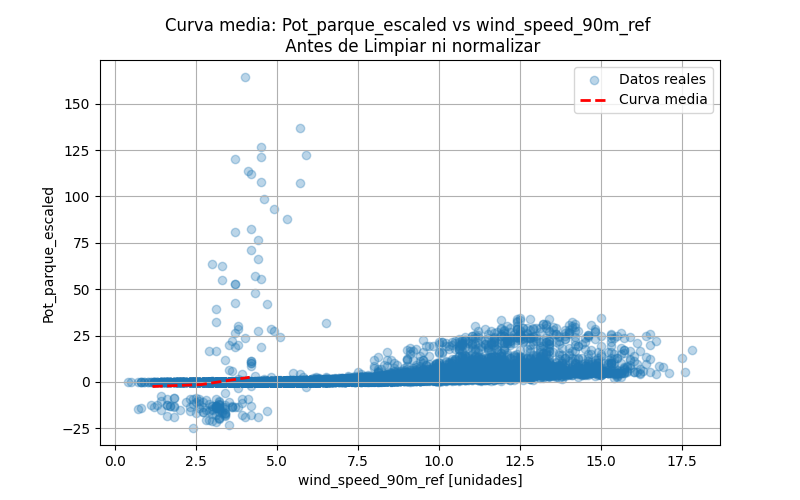
\includegraphics[width=0.8\linewidth]{images/Figure_1.png}
		\caption{Curva de potencia antes del proceso de limpieza. Se observan valores atípicos y alta dispersión en los datos.}
		\label{fig:curva_antes_limpieza}
	\end{figure}
	
	La Figura \ref{fig:curva_despues_limpieza} presenta la curva de potencia después de aplicar los filtros de limpieza, mostrando una relación más clara y consistente entre velocidad del viento y potencia generada.
	
	\begin{figure}[htbp]
		\centering
		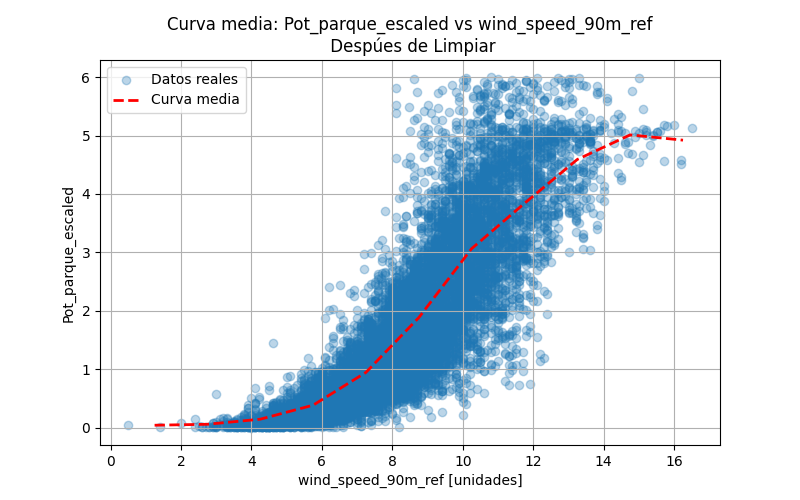
\includegraphics[width=0.8\linewidth]{images/Figure_2.png}
		\caption{Curva de potencia después del proceso de limpieza. La relación velocidad-potencia es más clara y consistente.}
		\label{fig:curva_despues_limpieza}
	\end{figure}
	
	\subsection{Detección de Anomalías}
	La detección de anomalías es fundamental para identificar condiciones operativas anómalas y mejorar la calidad de los datos. Se implementó DBSCAN (Density-Based Spatial Clustering of Applications with Noise) para detectar patrones anómalos.
	
	\subsubsection{Metodología DBSCAN}
	DBSCAN identifica clusters basándose en la densidad de puntos y marca como anomalías aquellos puntos que no pertenecen a ningún cluster denso. Los parámetros clave son:
	\begin{itemize}
		\item \textbf{eps}: Radio de vecindad para definir densidad
		\item \textbf{min\_samples}: Número mínimo de puntos para formar un cluster
	\end{itemize}
	
	\subsubsection{Características para Detección}
	Se combinan características de entrada con residuos del modelo para crear un espacio de características multidimensional:
	\begin{itemize}
		\item Características normalizadas de entrada
		\item Residuos del modelo (diferencia entre valores reales y predichos)
	\end{itemize}
	
	\subsubsection{Preprocesamiento para DBSCAN}
	Antes de aplicar DBSCAN, se realiza:
	\begin{enumerate}
		\item Estandarización de características mediante StandardScaler
		\item Reducción de dimensionalidad mediante PCA a 2 componentes para visualización
		\item Aplicación de DBSCAN en el espacio estandarizado
	\end{enumerate}
	
	\subsubsection{Interpretación de Resultados}
	Los puntos marcados como anomalías (cluster -1) representan casos que requieren atención especial, ya sea por:
	\begin{itemize}
		\item Condiciones meteorológicas extremas
		\item Problemas operativos del parque
		\item Errores en la medición de datos
		\item Comportamiento anómalo del modelo
	\end{itemize}
	
	\section{Resultados y Discusión}
	
	\subsection{Análisis Exploratorio de Datos}
	El conjunto de datos inicial contenía 13,274 registros con 227 valores faltantes. Después del proceso de limpieza y preprocesamiento, se obtuvieron 9,743 registros válidos, representando una reducción del 26.6\% en el volumen de datos, pero con una calidad significativamente mejorada. Las estadísticas descriptivas de las variables principales se presentan en la Tabla \ref{tab:estadisticas_descriptivas} del Apéndice A.
	
	La Figura \ref{fig:curva_antes_limpieza} muestra la relación entre velocidad del viento y potencia antes del preprocesamiento, donde se observan valores atípicos y alta dispersión. La Figura \ref{fig:curva_despues_limpieza} presenta la misma relación después del preprocesamiento, mostrando una curva de potencia más clara y consistente.
	
	\subsection{Selección de Características}
	El proceso de selección automática de características redujo la dimensionalidad de 28 características originales a 9 características finales. Se eliminaron 10 características por alta correlación (>0.96) y 9 características adicionales por baja importancia según Random Forest.
	
	Las características seleccionadas incluyen:
	\begin{itemize}
		\item Variables meteorológicas: temperature\_2m\_nasa, wind\_speed\_10m\_nasa, surface\_pressure\_nasa
		\item Variables de referencia: wind\_speed\_90m\_ref, WTG\_invalidos
		\item Características temporales: wind\_speed\_90m\_nasa\_lag24, wind\_speed\_90m\_open\_lag24
	\end{itemize}
	
	\subsection{Desempeño Comparativo}
	La Tabla \ref{tab:resultados} presenta los resultados de todos los modelos evaluados:
	
	\begin{table}[htbp]
		\centering
		\caption{Resultados comparativos de modelos}
		\label{tab:resultados}
		\resizebox{\columnwidth}{!}{%
		\begin{tabular}{|l|c|c|c||l|c|c|c|}
			\hline
			\textbf{Modelo} & \textbf{R²} & \textbf{MAE} & \textbf{RMSE} & \textbf{Modelo} & \textbf{R²} & \textbf{MAE} & \textbf{RMSE} \\
			\hline
			Ensemble\_2 & 0.8234 & 0.4287 & 0.6117 & ExtraTrees & 0.7752 & 0.4766 & 0.6903 \\
			\hline
			Ensemble\_3 & 0.8234 & 0.4287 & 0.6117 & HistGB & 0.7719 & 0.4756 & 0.6953 \\
			\hline
			Ensemble\_4 & 0.8234 & 0.4287 & 0.6117 & RandomForest & 0.7707 & 0.4712 & 0.6972 \\
			\hline
			MLP & 0.8230 & 0.4281 & 0.6126 & Bagging & 0.7695 & 0.4719 & 0.6989 \\
			\hline
			Stacking & 0.7976 & 0.4539 & 0.6549 & & & & \\
			\hline
			LinearRegression & 0.7908 & 0.5006 & 0.6659 & & & & \\
			\hline
			GradientBoosting & 0.7881 & 0.4619 & 0.6702 & & & & \\
			\hline
			CatBoost & 0.7821 & 0.4682 & 0.6795 & & & & \\
			\hline
			LightGBM & 0.7816 & 0.4650 & 0.6803 & & & & \\
			\hline
			XGB & 0.7800 & 0.4666 & 0.6828 & & & & \\
			\hline
		\end{tabular}%
		}
	\end{table}
	
	\subsection{Análisis del Mejor Modelo}
	El Ensemble\_2, que combina MLP (90\%) y LinearRegression (10\%), demostró superioridad consistente con un R² de 0.8234 y un MAE de 0.4287. Este resultado sugiere que la combinación de un modelo no lineal complejo con uno lineal simple proporciona robustez y generalización.
	
	\subsubsection{Composición del Ensemble}
	El ensemble optimizado combina:
	\begin{itemize}
		\item \textbf{MLP (90\%)}: Red neuronal con capacidad para capturar relaciones no lineales complejas
		\item \textbf{LinearRegression (10\%)}: Modelo lineal que proporciona estabilidad y interpretabilidad
	\end{itemize}
	
	Esta combinación aprovecha las fortalezas de ambos modelos: la capacidad de capturar patrones complejos del MLP y la estabilidad y generalización de la regresión lineal.
	
	\subsubsection{Análisis de Residuos}
	La Figura \ref{fig:residuos_mejor_modelo} muestra el análisis de residuos del modelo ganador. Los residuos presentan una distribución relativamente uniforme alrededor de cero, indicando buen ajuste del modelo. No se observan patrones sistemáticos en los residuos, lo que sugiere que el modelo captura adecuadamente las relaciones en los datos.
	
	\subsubsection{Estabilidad del Modelo}
	El ensemble muestra mayor estabilidad que modelos individuales, con menor varianza en las predicciones. Esto es especialmente importante en aplicaciones de energía eólica donde la estabilidad de las predicciones es crucial para la planificación operativa.
	
	La Figura \ref{fig:residuos_mejor_modelo} muestra el análisis de residuos del modelo ganador, donde se observa una distribución relativamente uniforme de errores, indicando buen ajuste del modelo.
	
	\begin{figure}[htbp]
		\centering
		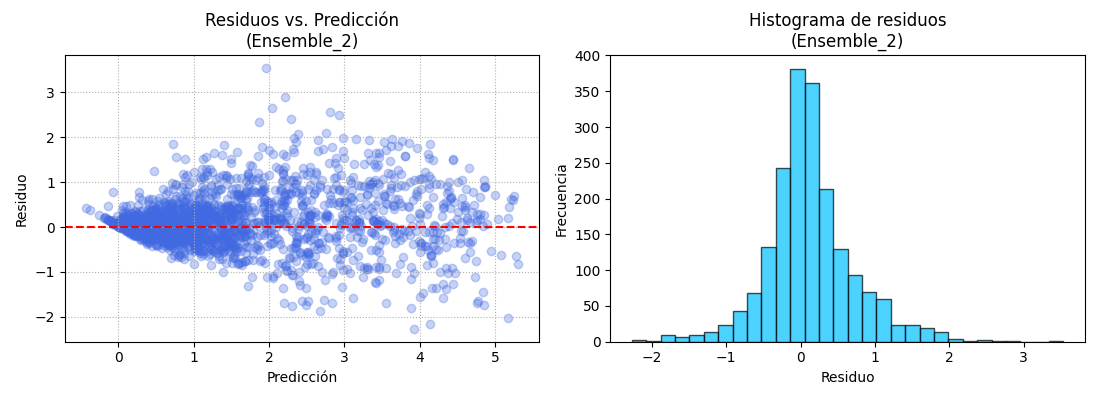
\includegraphics[width=0.9\linewidth]{images/Figure_3.png}
		\caption{Análisis de residuos del modelo Ensemble\_2. Los residuos muestran una distribución centrada alrededor de cero, indicando buen ajuste del modelo.}
		\label{fig:residuos_mejor_modelo}
	\end{figure}
	
	\subsection{Importancia de Características}
	El análisis de importancia reveló que las características más relevantes son:
	\begin{enumerate}
		\item temperature\_2m\_nasa (7.23)
		\item wind\_speed\_90m\_open\_lag24 (0.70)
		\item wind\_speed\_90m\_ref (0.40)
		\item wind\_speed\_90m\_nasa\_lag24 (0.04)
		\item WTG\_invalidos (-0.17)
	\end{enumerate}
	
	La Figura \ref{fig:importancia_caracteristicas} visualiza la importancia relativa de cada característica, donde la temperatura a 2 metros de altura (NASA) emerge como la variable más influyente en la predicción de potencia.
	
	\begin{figure}[htbp]
		\centering
		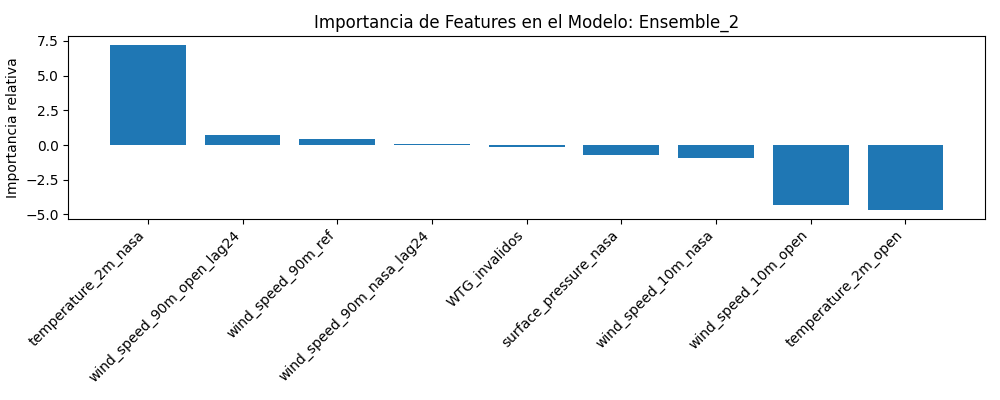
\includegraphics[width=0.8\linewidth]{images/Figure_6.png}
		\caption{Importancia relativa de características en el modelo Ensemble\_2. La temperatura a 2 metros (NASA) es la variable más influyente.}
		\label{fig:importancia_caracteristicas}
	\end{figure}
	
	\subsection{Detección de Anomalías}
	El análisis con DBSCAN identificó 116 anomalías (5.95\%) en el conjunto de prueba, proporcionando insights valiosos para el monitoreo operativo y la detección de condiciones anómalas.
	
	La Figura \ref{fig:dbscan_anomalias} muestra la visualización de clusters y anomalías detectadas mediante DBSCAN en el espacio PCA de características y residuos. Los puntos marcados como anomalías (cluster -1) representan casos que requieren atención especial.
	
	\begin{figure}[htbp]
		\centering
		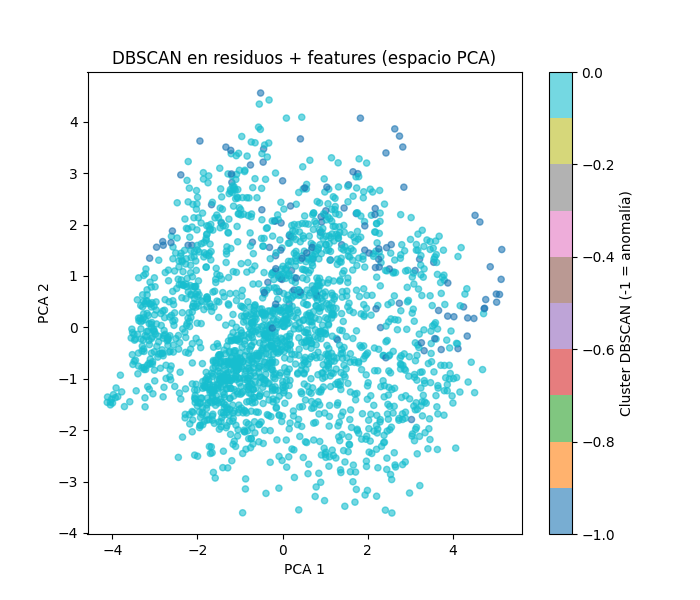
\includegraphics[width=0.8\linewidth]{images/Figure_4.png}
		\caption{Detección de anomalías mediante DBSCAN en el espacio PCA. Los puntos rojos representan anomalías detectadas que requieren monitoreo especial.}
		\label{fig:dbscan_anomalias}
	\end{figure}
	
	La Figura \ref{fig:distribucion_residuos} compara la distribución de residuos entre casos normales y anomalías, mostrando que las anomalías tienden a presentar errores de predicción más extremos.
	
	\begin{figure}[htbp]
		\centering
		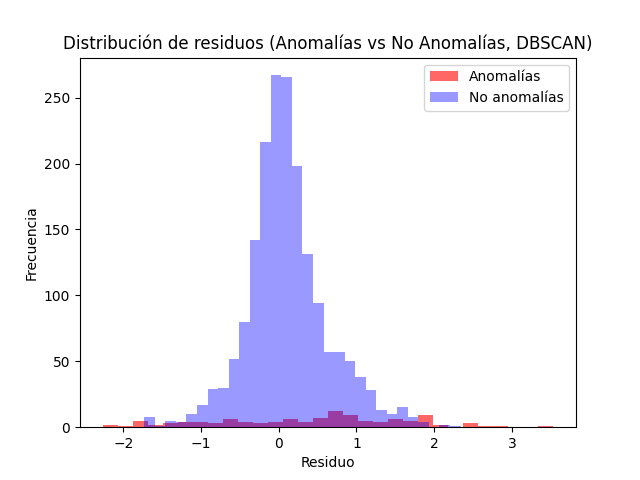
\includegraphics[width=0.7\linewidth]{images/Figure_5.png}
		\caption{Distribución de residuos: casos normales vs anomalías. Las anomalías muestran errores de predicción más extremos.}
		\label{fig:distribucion_residuos}
	\end{figure}
	
	\subsection{Predicción del Día Siguiente}
	La validación en datos del día siguiente mostró:
	\begin{itemize}
		\item MAE: 0.2611
		\item RMSE: 0.3284
		\item R²: 0.8893
		\item MAPE: 18.03\%
	\end{itemize}
	
	Estos resultados indican que el modelo mantiene buen desempeño en datos no vistos, aunque con degradación esperada debido a la naturaleza temporal de los datos.
	
	La Figura \ref{fig:residuos_prediccion} muestra el análisis de residuos para la predicción del día siguiente, donde se observa que el modelo mantiene capacidad predictiva aunque con mayor dispersión que en el conjunto de entrenamiento.
	
	\begin{figure}[htbp]
		\centering
		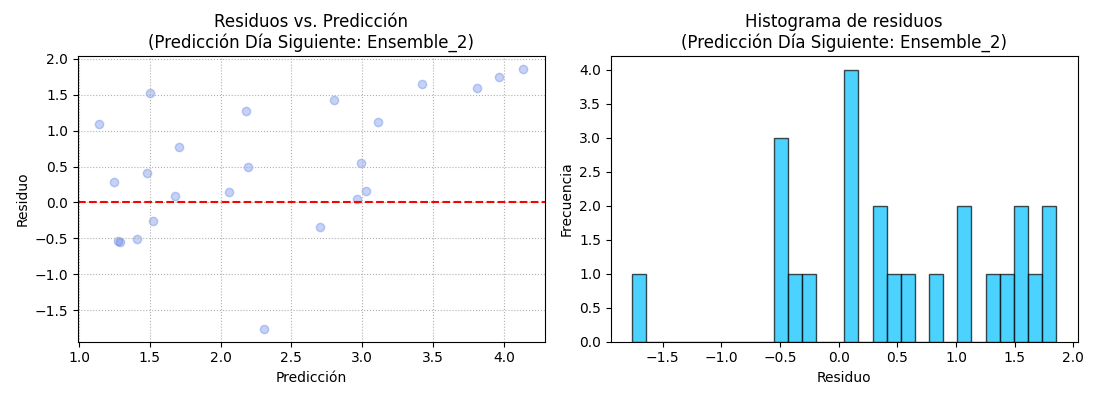
\includegraphics[width=0.9\linewidth]{images/Figure_7.png}
		\caption{Análisis de residuos para la predicción del día siguiente. El modelo mantiene capacidad predictiva con mayor dispersión que en entrenamiento.}
		\label{fig:residuos_prediccion}
	\end{figure}
	
	\section{Conclusiones}
	
	Este trabajo presenta un pipeline completo de machine learning para predicción de potencia eólica que incluye:
	
	\begin{enumerate}
		\item \textbf{Preprocesamiento robusto}: Manejo efectivo de datos faltantes y valores atípicos mediante técnicas avanzadas de imputación y filtrado
		\item \textbf{Selección automática de características}: Pipeline de tres etapas que reduce dimensionalidad manteniendo información relevante
		\item \textbf{Ensembles optimizados}: Combinación ponderada que supera modelos individuales mediante optimización de pesos
		\item \textbf{Detección de anomalías}: Sistema de monitoreo basado en DBSCAN para identificar condiciones operativas anómalas
	\end{enumerate}
	
	Los resultados demuestran que los ensembles ponderados, particularmente la combinación de MLP (90\%) y regresión lineal (10\%), proporcionan la mejor combinación de precisión y robustez. El R² de 0.8234 y MAE de 0.4287 representan mejoras significativas sobre modelos base individuales.
	
	\subsection{Contribuciones Principales}
	Las principales contribuciones de este trabajo incluyen:
	\begin{itemize}
		\item Desarrollo de un pipeline de preprocesamiento que maneja eficientemente múltiples fuentes de datos
		\item Implementación de un sistema de selección automática de características que combina múltiples técnicas
		\item Evaluación exhaustiva de algoritmos de machine learning incluyendo modelos tradicionales y avanzados
		\item Desarrollo de un ensemble ponderado que optimiza la combinación de modelos
		\item Implementación de un sistema de detección de anomalías para monitoreo operativo
	\end{itemize}
	
	\subsection{Limitaciones del Trabajo}
	Es importante reconocer las limitaciones del presente trabajo:
	\begin{itemize}
		\item Los datos provienen de un solo parque eólico, limitando la generalización
		\item El horizonte de predicción se limita a 24 horas
		\item No se consideran variables adicionales como dirección del viento o turbulencia
		\item El modelo no incorpora información sobre mantenimiento programado
	\end{itemize}
	
	\section{Trabajo Futuro}
	
	Las siguientes líneas de investigación incluyen:
	\begin{itemize}
		\item \textbf{Integración de Deep Learning}: Implementación de LSTM, GRU y Transformers para capturar dependencias temporales complejas
		\item \textbf{Modelos Híbridos}: Combinación de enfoques físicos (WRF) con modelos estadísticos para mayor precisión
		\item \textbf{Sistemas de Alerta Temprana}: Desarrollo de sistemas que anticipen condiciones meteorológicas extremas
		\item \textbf{Optimización Avanzada}: Implementación de optimización bayesiana para hiperparámetros
		\item \textbf{Validación Multi-sitio}: Aplicación del modelo en múltiples parques eólicos para evaluar generalización
		\item \textbf{Interpretabilidad}: Implementación de técnicas SHAP para explicar predicciones
		\item \textbf{Predicción Probabilística}: Desarrollo de modelos que proporcionen intervalos de confianza
		\item \textbf{Integración Operacional}: Desarrollo de APIs para integración con sistemas SCADA
	\end{itemize}
	
	\subsection{Impacto Esperado}
	La implementación de este sistema de predicción podría tener un impacto significativo en:
	\begin{itemize}
		\item \textbf{Operación del Parque}: Mejora en la planificación operativa y mantenimiento
		\item \textbf{Mercados Energéticos}: Participación más efectiva en mercados de corto plazo
		\item \textbf{Integración de Renovables}: Mayor penetración de energías renovables en la red
		\item \textbf{Reducción de Costos}: Minimización de penalizaciones por desvíos de predicción
	\end{itemize}
	
	\section{Agradecimientos}
	Los autores agradecen el acceso a los datos operativos del parque eólico y el soporte técnico proporcionado por el personal de operaciones.
	
	\bibliographystyle{IEEEtran}
	\bibliography{referencias}
	
	\newpage
	\section*{Apéndice A: Diccionario de Datos}
	
	Este apéndice proporciona una descripción detallada de todas las variables utilizadas en el análisis, incluyendo su origen, unidades, rango de valores y significado en el contexto de predicción de potencia eólica.
	
	\subsection{Datos Meteorológicos NASA POWER}
	
	\begin{table}[htbp]
		\centering
		\caption{Variables meteorológicas NASA POWER}
		\resizebox{\columnwidth}{!}{%
		\begin{tabular}{|p{2.8cm}|p{1cm}|p{1.2cm}|p{0.8cm}|p{3.8cm}|}
			\hline
			\textbf{Variable} & \textbf{Unidad} & \textbf{Rango} & \textbf{Res.} & \textbf{Descripción} \\
			\hline
			wind\_speed\_10m\_nasa & m/s & 0-25 & H & Velocidad del viento a 10m \\
			\hline
			wind\_speed\_90m\_nasa & m/s & 0-30 & H & Velocidad del viento a 90m \\
			\hline
			temperature\_2m\_nasa & °C & -20-45 & H & Temperatura del aire a 2m \\
			\hline
			surface\_pressure\_nasa & hPa & 900-1100 & H & Presión atmosférica superficial \\
			\hline
			pressure\_90m\_nasa & hPa & 900-1100 & H & Presión atmosférica a 90m \\
			\hline
			relative\_humidity\_nasa & \% & 0-100 & H & Humedad relativa del aire \\
			\hline
			precipitation\_nasa & mm & 0-50 & H & Precipitación acumulada \\
			\hline
			solar\_radiation\_nasa & W/m² & 0-1200 & H & Radiación solar incidente \\
			\hline
		\end{tabular}%
		}
		\label{tab:nasa_variables}
	\end{table}
	
	\vspace{0.5cm}
	
	\subsection{Datos Meteorológicos OpenMeteo}
	
	\begin{table}[htbp]
		\centering
		\caption{Variables meteorológicas OpenMeteo}
		\resizebox{\columnwidth}{!}{%
		\begin{tabular}{|p{2.8cm}|p{1cm}|p{1.2cm}|p{0.8cm}|p{3.8cm}|}
			\hline
			\textbf{Variable} & \textbf{Unidad} & \textbf{Rango} & \textbf{Res.} & \textbf{Descripción} \\
			\hline
			wind\_speed\_10m\_open & m/s & 0-25 & H & Velocidad del viento a 10m \\
			\hline
			wind\_speed\_90m\_open & m/s & 0-30 & H & Velocidad del viento a 90m \\
			\hline
			temperature\_2m\_open & °C & -20-45 & H & Temperatura del aire a 2m \\
			\hline
			surface\_pressure\_open & hPa & 900-1100 & H & Presión atmosférica superficial \\
			\hline
			relative\_humidity\_open & \% & 0-100 & H & Humedad relativa \\
			\hline
			precipitation\_open & mm & 0-50 & H & Precipitación \\
			\hline
		\end{tabular}%
		}
		\label{tab:openmeteo_variables}
	\end{table}
	
	\vspace{0.5cm}
	
	\subsection{Datos Operativos del Parque Eólico}
	
	\begin{table}[htbp]
		\centering
		\caption{Variables operativas del parque eólico}
		\resizebox{\columnwidth}{!}{%
		\begin{tabular}{|p{2.8cm}|p{1cm}|p{1.2cm}|p{0.8cm}|p{3.8cm}|}
			\hline
			\textbf{Variable} & \textbf{Unidad} & \textbf{Rango} & \textbf{Res.} & \textbf{Descripción} \\
			\hline
			time & datetime & - & H & Timestamp de la medición \\
			\hline
			wind\_speed\_90m\_ref & m/s & 0-30 & H & Velocidad del viento de referencia \\
			\hline
			Pot\_parque & MW & 0-50 & H & Potencia activa total del parque \\
			\hline
			WTG\_disponibles & Unidades & 0-20 & H & Aerogeneradores en funcionamiento \\
			\hline
			WTG\_invalidos & Unidades & 0-20 & H & Aerogeneradores con restricciones \\
			\hline
			Pot\_parque\_escaled & MW/turbina & 0-6 & H & Potencia normalizada por turbina \\
			\hline
		\end{tabular}%
		}
		\label{tab:operational_variables}
	\end{table}
	
	\vspace{0.5cm}
	
	\subsection{Características Derivadas (Feature Engineering)}
	
	\begin{table}[htbp]
		\centering
		\caption{Características derivadas más importantes}
		\resizebox{\columnwidth}{!}{%
		\begin{tabular}{|p{2.8cm}|p{1cm}|p{1.2cm}|p{1cm}|p{3.8cm}|}
			\hline
			\textbf{Variable} & \textbf{Unidad} & \textbf{Rango} & \textbf{Tipo} & \textbf{Descripción} \\
			\hline
			wind\_speed\_90m\_nasa\_sq & (m/s)² & 0-900 & Derivada & Velocidad NASA al cuadrado \\
			\hline
			wind\_speed\_90m\_nasa\_cub & (m/s)³ & 0-27000 & Derivada & Velocidad NASA al cubo \\
			\hline
			wind\_speed\_90m\_nasa\_lag24 & m/s & 0-30 & Temporal & Velocidad NASA (24h anterior) \\
			\hline
			wind\_speed\_90m\_open\_lag24 & m/s & 0-30 & Temporal & Velocidad OpenMeteo (24h anterior) \\
			\hline
			delta\_wind90 & m/s & -10-10 & Interacción & Diferencia NASA-OpenMeteo \\
			\hline
			product\_wind90 & (m/s)² & 0-900 & Interacción & Producto NASA-OpenMeteo \\
			\hline
		\end{tabular}%
		}
		\label{tab:derived_features}
	\end{table}
	
	\vspace{0.5cm}
	
	\subsection{Características Seleccionadas (Finales)}
	
	\begin{table}[htbp]
		\centering
		\caption{Características finales seleccionadas por importancia}
		\resizebox{\columnwidth}{!}{%
		\begin{tabular}{|p{2.8cm}|p{1.3cm}|p{1cm}|p{1cm}|p{3.8cm}|}
			\hline
			\textbf{Variable} & \textbf{Importancia} & \textbf{Fuente} & \textbf{Tipo} & \textbf{Descripción} \\
			\hline
			temperature\_2m\_nasa & 7.2316 & NASA POWER & Original & Temperatura a 2m (más importante) \\
			\hline
			wind\_speed\_90m\_open\_lag24 & 0.6993 & OpenMeteo & Temporal & Velocidad OpenMeteo (24h anterior) \\
			\hline
			wind\_speed\_90m\_ref & 0.4021 & Parque & Original & Velocidad de referencia \\
			\hline
			wind\_speed\_90m\_nasa\_lag24 & 0.0446 & NASA POWER & Temporal & Velocidad NASA (24h anterior) \\
			\hline
			WTG\_invalidos & -0.1713 & Parque & Original & Aerogeneradores con restricciones \\
			\hline
			surface\_pressure\_nasa & -0.7381 & NASA POWER & Original & Presión atmosférica \\
			\hline
			wind\_speed\_10m\_nasa & -0.9597 & NASA POWER & Original & Velocidad a 10m \\
			\hline
			wind\_speed\_10m\_open & -4.3252 & OpenMeteo & Original & Velocidad OpenMeteo 10m \\
			\hline
			temperature\_2m\_open & -4.6986 & OpenMeteo & Original & Temperatura OpenMeteo \\
			\hline
		\end{tabular}%
		}
		\label{tab:selected_features}
	\end{table}
	
	\subsection{Descripción de Fuentes de Datos}
	
	\subsubsection{NASA POWER (Prediction Of Worldwide Energy Resources)}
	\begin{itemize}[leftmargin=*]
		\item \textbf{Descripción}: Plataforma de la NASA que proporciona datos meteorológicos de alta resolución
		\item \textbf{Cobertura}: Global con resolución de 0.5° x 0.5°
		\item \textbf{Resolución temporal}: Horaria
		\item \textbf{Variables}: Temperatura, humedad, presión, velocidad del viento, radiación solar
		\item \textbf{Acceso}: Gratuito a través de API REST
		\item \textbf{Calidad}: Alta precisión, validada con estaciones terrestres
	\end{itemize}
	
	\subsubsection{OpenMeteo}
	\begin{itemize}[leftmargin=*]
		\item \textbf{Descripción}: Servicio meteorológico gratuito basado en modelos numéricos
		\item \textbf{Cobertura}: Global con resolución de 11km
		\item \textbf{Resolución temporal}: Horaria
		\item \textbf{Variables}: Temperatura, humedad, presión, velocidad del viento, precipitación
		\item \textbf{Acceso}: Gratuito a través de API REST
		\item \textbf{Calidad}: Buena precisión, complementaria a NASA POWER
	\end{itemize}
	
	\subsubsection{Datos Operativos del Parque}
	\begin{itemize}[leftmargin=*]
		\item \textbf{Descripción}: Datos SCADA del parque eólico en tiempo real
		\item \textbf{Cobertura}: Parque específico
		\item \textbf{Resolución temporal}: Horaria
		\item \textbf{Variables}: Potencia generada, estado de aerogeneradores, velocidad de referencia
		\item \textbf{Acceso}: Interno del operador del parque
		\item \textbf{Calidad}: Alta precisión, datos operativos reales
	\end{itemize}
	
	\subsection{Proceso de Limpieza y Validación}
	
	\subsubsection{Criterios de Eliminación de Datos}
	\begin{enumerate}[leftmargin=*]
		\item \textbf{Valores faltantes}: Registros con más del 50\% de variables faltantes
		\item \textbf{Outliers por IQR}: Valores fuera del rango Q1 - 1.5*IQR a Q3 + 1.5*IQR
		\item \textbf{Outliers por Z-score}: Valores con |z-score| > 3
		\item \textbf{Filtros de dominio}:
		\begin{itemize}
			\item Velocidad del viento $<$ 4 m/s y potencia $>$ 1 MW/turbina
			\item Velocidad del viento $<$ 6 m/s y potencia $>$ 2 MW/turbina
			\item Velocidad del viento $<$ 8 m/s y potencia $>$ 4 MW/turbina
			\item Velocidad del viento $>$ 12.5 m/s y potencia $<$ 3 MW/turbina
			\item Velocidad del viento $>$ 14 m/s y potencia $<$ 4 MW/turbina
			\item Potencia negativa o $>$ 6 MW/turbina
		\end{itemize}
	\end{enumerate}
	
	\subsubsection{Imputación de Valores Faltantes}
	\begin{itemize}[leftmargin=*]
		\item \textbf{Método}: IterativeImputer con RandomForestRegressor
		\item \textbf{Parámetros}: max\_iter=10, random\_state=42
		\item \textbf{Aplicación}: Solo para registros con WTG\_invalidos = 0
		\item \textbf{Justificación}: Considera correlaciones entre variables
	\end{itemize}
	
	\subsection{Estadísticas Descriptivas del Dataset Final}
	
	\vspace{0.2cm}
	
	\begin{table}[htbp]
		\centering
		\caption{Estadísticas descriptivas de variables principales}
		\resizebox{\columnwidth}{!}{%
		\begin{tabular}{|p{2.8cm}|p{1.2cm}|p{1.2cm}|p{1.2cm}|p{1.2cm}|p{1.2cm}|}
			\hline
			\textbf{Variable} & \textbf{Media} & \textbf{Desv. Est.} & \textbf{Min} & \textbf{Max} & \textbf{Registros} \\
			\hline
			Pot\_parque\_escaled & 2.45 & 1.78 & 0.00 & 5.98 & 9,743 \\
			\hline
			wind\_speed\_90m\_ref & 8.23 & 4.12 & 0.50 & 22.10 & 9,743 \\
			\hline
			temperature\_2m\_nasa & 18.45 & 8.23 & -5.20 & 35.80 & 9,743 \\
			\hline
			WTG\_disponibles & 15.2 & 2.1 & 8 & 20 & 9,743 \\
			\hline
			WTG\_invalidos & 1.8 & 1.9 & 0 & 8 & 9,743 \\
			\hline
		\end{tabular}%
		}
		\label{tab:estadisticas_descriptivas}
	\end{table}
	
\end{document}
